\section{结果}

\subsection{完整规模主结果比较}

表~\ref{tab:main-results-zh} 报告四个预测时域上的宏平均结果。

\begin{table}[!t]
\centering
\small
\resizebox{\textwidth}{!}{%
\begin{tabular}{lcccccccccc}
\toprule
模型 & Top1 & Top3 & Top5 & NLL & Brier & ECE & Union Cover & Union Cells & Union Area km$^2$ & Cover@Budget \\
\midrule
Markov 基线 & 0.3184 & 0.6166 & 0.7587 & 2.2788 & 0.8111 & 0.0323 & 0.8749 & 9.9542 & 545174 & 0.9699 \\
层级 GRU & 0.6648 & 0.9076 & 0.9631 & 1.0214 & 0.4578 & 0.0180 & 0.8931 & 2.4189 & 128965 & 0.9980 \\
TrAISformer-H3 & 0.6803 & \textbf{0.9178} & \textbf{0.9697} & \textbf{0.9556} & 0.4361 & 0.0094 & \textbf{0.8939} & 2.2297 & 122810 & \textbf{0.9983} \\
FlightBERT++-H3 & 0.6764 & 0.9144 & 0.9671 & 0.9791 & 0.4417 & \textbf{0.0086} & 0.8883 & 2.2023 & \textbf{117593} & 0.9982 \\
Transformer horizon decoder & 0.6744 & 0.9129 & 0.9656 & 0.9946 & 0.4447 & 0.0123 & 0.8920 & 2.2721 & 122553 & 0.9981 \\
\textbf{所提出的多尺度模型} & \textbf{0.6827} & 0.9174 & 0.9685 & 0.9641 & \textbf{0.4338} & 0.0093 & 0.8922 & \textbf{2.1829} & 118810 & 0.9983 \\
\bottomrule
\end{tabular}

}
\caption{10、30、60 和 120 分钟预测时域上的完整规模宏平均比较。}
\label{tab:main-results-zh}
\end{table}

\begin{figure}[!t]
\centering
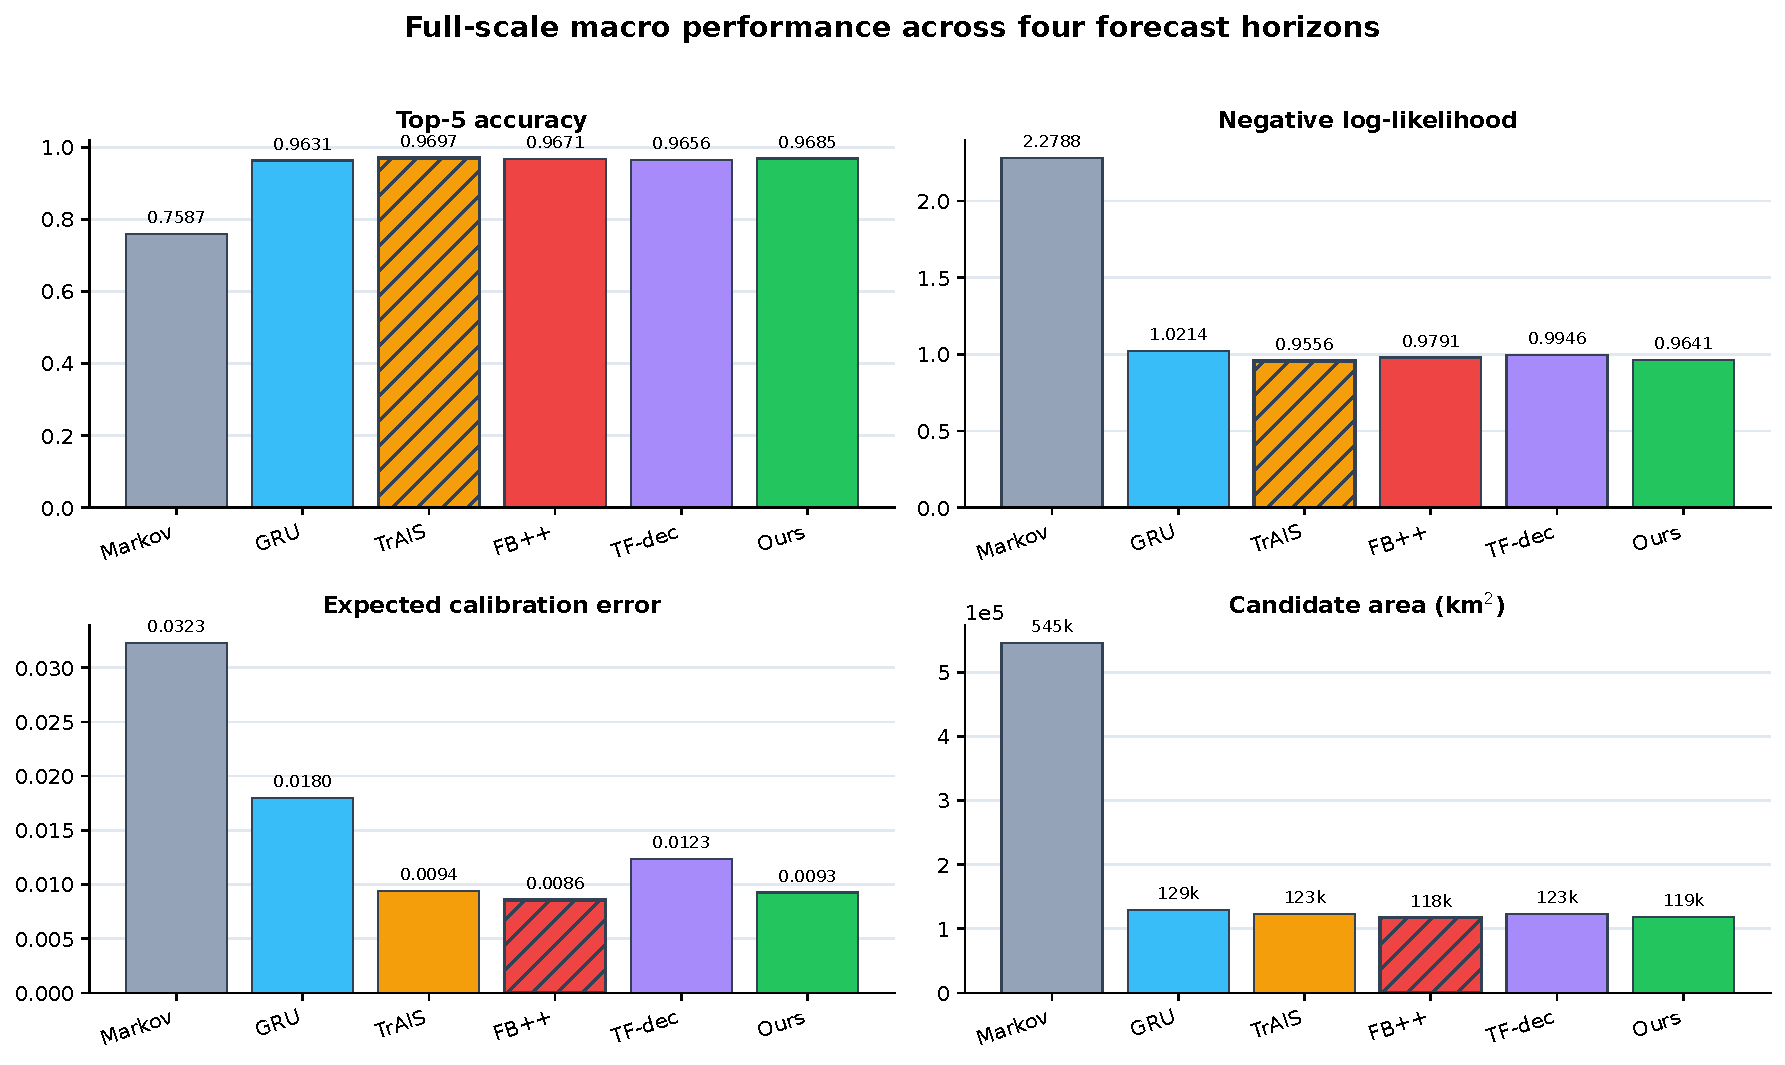
\includegraphics[width=\textwidth]{figures/fig2_main_results_overview.pdf}
\caption{完整规模主结果概览。相较内部基线和两个外部适配基线，所提出的多尺度模型在 top-1、Brier 分数和候选集合紧致性上保持整体最优平衡。}
\label{fig:main-results-overview-zh}
\end{figure}

结果有三点值得注意。首先，所有学习型层级模型都显著优于经典 Markov 基线。其次，在两个外部适配基线中，TrAISformer-H3 是最强竞争者：它取得最高的宏平均 top-3/top-5、最低的 NLL，以及最高的 union cover。第三，所提出的多尺度模型仍然保持最佳宏平均 top-1（0.6827）、最佳 Brier 分数（0.4338）和最小的 candidate union cell 数（2.1829），说明它在分类正确性、概率质量和候选集合紧致性之间取得了更均衡的折中。

FlightBERT++-H3 呈现另一种行为模式。它的宏平均 ECE 最低（0.0086），候选 union 面积也最小（117,593 km$^2$），但 top-1/top-3/top-5 和 union cover 均低于所提模型。这说明更保守、更紧的候选集合并不自动意味着更好的整体区域预测；如果排序能力下降，候选覆盖也会同步退化。

从逐时域结果看，TrAISformer-H3 在 10 和 30 分钟时域上略优于所提模型的 top-3/top-5，但在 120 分钟时域上，所提模型重新取得明显优势：top-1 从 0.5481 提升到 0.5565，top-3 从 0.8482 提升到 0.8531，top-5 从 0.9355 提升到 0.9372，同时 NLL、Brier 和 ECE 也全部更优。这一现象支持本文的核心判断：显式多尺度时间建模的价值主要体现在中长时域区域预测，而不是只在短时排序指标上获益。

\subsection{相较层级 GRU 基线的提升}

相较层级 GRU 基线，所提模型提升了所有 top-k 指标和所有概率指标：top-1 从 0.6648 提升到 0.6827，top-3 从 0.9076 提升到 0.9174，top-5 从 0.9631 提升到 0.9685；NLL 从 1.0214 降至 0.9641，Brier 分数从 0.4578 降至 0.4338，ECE 从 0.0180 降至 0.0093。

提升在不同预测时域上具有一致性。表~\ref{tab:delta-gru-zh} 给出了相较 GRU 基线的逐时域差值。

\begin{table}[!t]
\centering
\small
\resizebox{\textwidth}{!}{%
\begin{tabular}{cccccccccc}
\toprule
时域 & $\Delta$Top1 & $\Delta$Top3 & $\Delta$Top5 & $\Delta$NLL & $\Delta$Brier & $\Delta$ECE & $\Delta$Union Cover & $\Delta$Union Cells & $\Delta$Union Area km$^2$ \\
\midrule
10m & +0.0199 & +0.0059 & +0.0031 & -0.0516 & -0.0281 & -0.0085 & -0.0004 & -0.1864 & -2316 \\
30m & +0.0214 & +0.0129 & +0.0076 & -0.0759 & -0.0303 & -0.0210 & -0.0052 & -0.3683 & -4567 \\
60m & +0.0115 & +0.0054 & +0.0018 & -0.0340 & -0.0158 & -0.0016 & +0.0023 & -0.0908 & -7705 \\
120m & +0.0190 & +0.0153 & +0.0091 & -0.0674 & -0.0220 & -0.0040 & -0.0005 & -0.2988 & -26031 \\
\bottomrule
\end{tabular}

}
\caption{所提模型相较层级 GRU 基线的逐时域差值。对于 top-k 和 union cover，正值更好；对于 NLL、Brier、ECE、候选 cell 和候选面积，负值更好。}
\label{tab:delta-gru-zh}
\end{table}

\subsection{结构消融：多尺度分支是否必要}

为了分离显式多尺度时间编码的价值，我们将最终模型与单尺度 Transformer horizon decoder 比较。后者已经具有时域专属 query，但不包含多尺度分支。

\begin{table}[!t]
\centering
\small
\resizebox{\textwidth}{!}{%
\begin{tabular}{lccccc}
\toprule
模型 & Top1 & Top5 & NLL & Brier & ECE \\
\midrule
Transformer horizon decoder & 0.6744 & 0.9656 & 0.9946 & 0.4447 & 0.0123 \\
Multiscale Transformer & 0.6827 & 0.9685 & 0.9641 & 0.4338 & \textbf{0.0093} \\
\textbf{Horizon-Router} & \textbf{0.6884} & \textbf{0.9710} & \textbf{0.9399} & \textbf{0.4262} & 0.0104 \\
\bottomrule
\end{tabular}

}
\caption{单尺度 Transformer horizon decoder 与所提出多尺度模型的结构消融比较。}
\label{tab:structural-ablation-zh}
\end{table}

多尺度分支改善了所有主要宏平均指标，并取得更低的验证损失（0.3055 对 0.3177）。这支持本文判断：显式双尺度时间建模带来的收益，并不只是把 GRU 替换为 Transformer 所能解释。

\subsection{H3 邻域 refinement 体现召回与校准的权衡}

接着，我们在三个扩散强度上评估 H3 邻域 refinement。该策略提高了概率质量候选召回，但不是无代价收益。

\begin{table}[!t]
\centering
\small
\resizebox{\textwidth}{!}{%
\begin{tabular}{lcccccccc}
\toprule
模型 & Top5 & NLL & Brier & ECE & Union Cover & Union Cells & Union Area km$^2$ & Cover@Budget \\
\midrule
最终模型 & 0.9685 & 0.9641 & 0.4338 & 0.0093 & 0.8922 & 2.1829 & 118810 & 0.9983 \\
Refine a=0.05 & 0.9677 & 0.9593 & 0.4344 & 0.0310 & 0.9052 & 2.3315 & 127062 & 0.9987 \\
Refine a=0.10 & 0.9673 & 0.9796 & 0.4372 & 0.0585 & 0.9192 & 2.5168 & 137220 & 0.9987 \\
Refine a=0.20 & 0.9662 & 1.0340 & 0.4493 & 0.1135 & 0.9496 & 3.0980 & 167889 & 0.9987 \\
\bottomrule
\end{tabular}

}
\caption{完整数据集上的 H3 邻域 refinement sweep。更高的 union cover 伴随更差的校准性和更大的候选集合。}
\label{tab:h3-refine-zh}
\end{table}

\begin{figure}[!t]
\centering
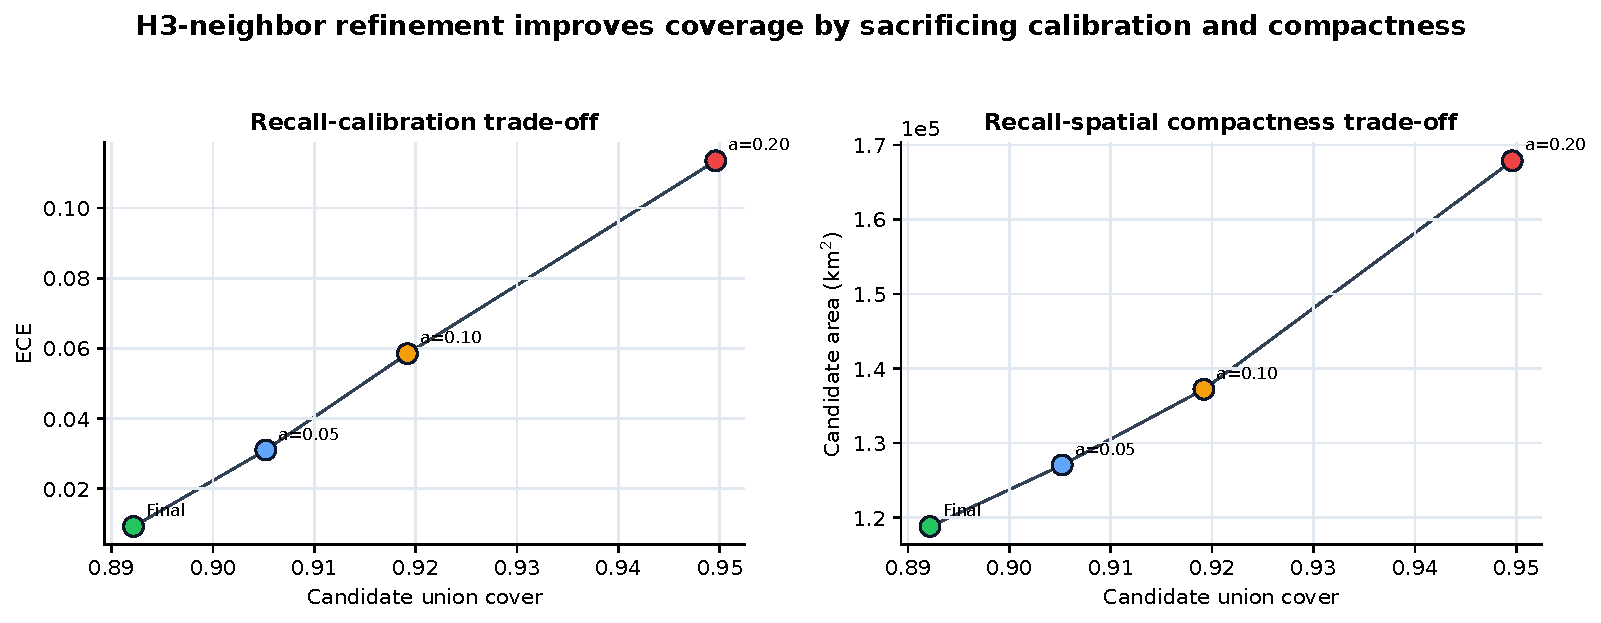
\includegraphics[width=0.78\textwidth]{figures/fig3_h3_refinement_tradeoff.pdf}
\caption{H3 邻域 refinement 提高候选 union cover，但额外召回以更差校准性和更大空间候选面积为代价。}
\label{fig:h3-refinement-tradeoff-zh}
\end{figure}

refinement 提高了候选 union cover，但很快损害校准性，并最终恶化 top-5 和 NLL。因此，它不应作为最终模型呈现。它的价值在于揭示一个具有运行意义的权衡：本地空间平滑可以提高召回，但会牺牲置信度质量和空间紧凑性。

\subsection{Reachability filtering 的聚合影响较小}

关闭 reachability filtering 只带来很小的聚合指标变化。这说明在当前设置中，reachability filtering 更像是一个可达性合理性保护，而不是预测收益的主要来源。
